%   ------------------------------------------------------------------------
\FloatBarrier
\section{Análise do Pixel Lab}
\label{s.pixelLab}

A plataforma Pixel Lab foi selecionada por seu foco em pixel art, com diversas funcionalidades para o auxílio na criação e refinamento da animação, como:

\begin{itemize}
    \item Ferramenta de rotação;
    \item Animação para animação; e
    \item Edição de imagem.
\end{itemize}


A ferramenta também possui a capacidade de gerar os movimentos de um personagem através do sistema de animação baseado no esqueleto, porém esse recurso não pôde ser testado por ser pago. 

Além disso, existe um editor embutido especificamente para pixel art no ambiente da geração, sendo possível fazer a edição de pixels específicos e tendo outras funcionalidades básicas para a criação e edição de sprites. Esse editor possui uma separação de quadros da animação, podendo receber diretamente o sprite sheet e separar cada uma das imagens em seu respectivo frame, além de também conseguir exportar esse sprite sheet em diversos formatos, com números variados de linhas e colunas (Figura \ref{fig:pixelLabExport} no Apêndice \ref{ap.telasIA}). Apesar de não formar nenhum vídeo diretamente, a ferramenta consegue tocar a animação, considerando todos os quadros ou aqueles pertencentes a uma tag (Figura \ref{fig:pixelLabViewAnimation} no Apêndice \ref{ap.telasIA}). Uma tag pode ser criada clicando com o botão direito do mouse nos números dos frames e selecionando a opção new tag (nova tag, em inglês).

Foi realizado uma série de testes dentro da ferramenta, grande parte deles visando auxiliar na pré-produção de uma animação, (criando imagens de referência), ou no ajuste fino e edições finais do resultado gerado por outra ferramenta.


%%% pablo, pablo lateral de alguma IA, ver tudo que pegou de fora
\begin{figure}[htbp]
    \centering
    \caption{\small Artefatos usados para referência no Pixel Lab}
    \label{fig:pixelLabArtefatos}
    \begin{subfigure}{0.32\linewidth}
        
\includegraphics[width=0.7\linewidth]{figs/sprites/Pablo.PNG}
        \caption{\small Sprite do personagem Pablo em front view}
        \label{fig:pixelLabPablo}
    \end{subfigure}
    \begin{subfigure}{0.32\linewidth}
        
\includegraphics[width=1\linewidth]{figs/sprites/irma.png}
        \caption{\small Sprite da personagem Luz}
        \label{fig:pixelLabIrma}
    \end{subfigure}
    \begin{subfigure}{1\linewidth}
        \centering
        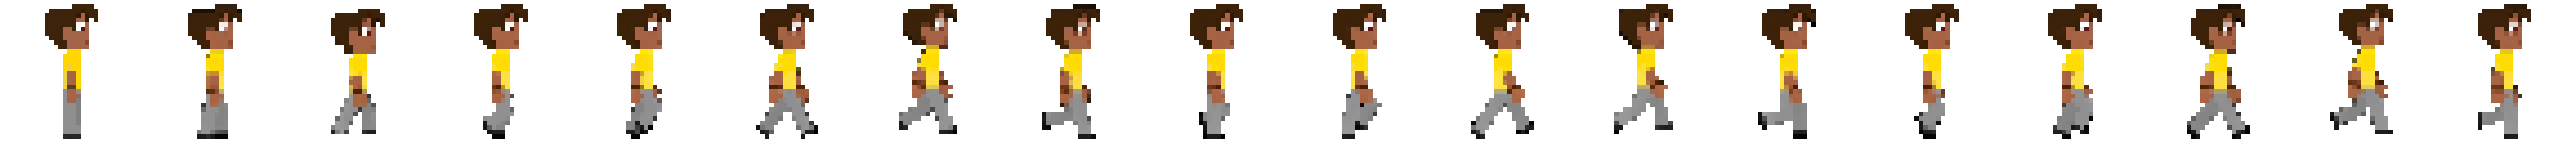
\includegraphics[width=1\linewidth]{figs/geminiPro/walking_sprite_sheet_grande_pixel.png}
        \caption{\small Sprite sheet gerado pelo Gemini Pro}
        \label{fig:pixelLabSpriteSheetGeminiPro}
    \end{subfigure}
    \begin{subfigure}{1\linewidth}
        \centering
        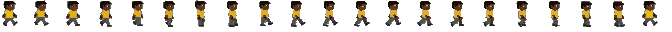
\includegraphics[width=1\linewidth]{figs/godmodAI/Pixilart/pixilart-sprite.png}
        \caption{\small Sprite sheet gerado pelo God Mode AI}
        \label{fig:pixelLabSpriteSheetGodModeAI}
    \end{subfigure}
    \legend{\small Fonte: Elaborada pela autora.}
\end{figure}

\begin{figure}[htbp]
    \centering
    \caption{\small Artefatos editados no Pixel Lab}
    \label{fig:pixelLabEdicao}
    \begin{subfigure}{0.45\linewidth}
        \centering
        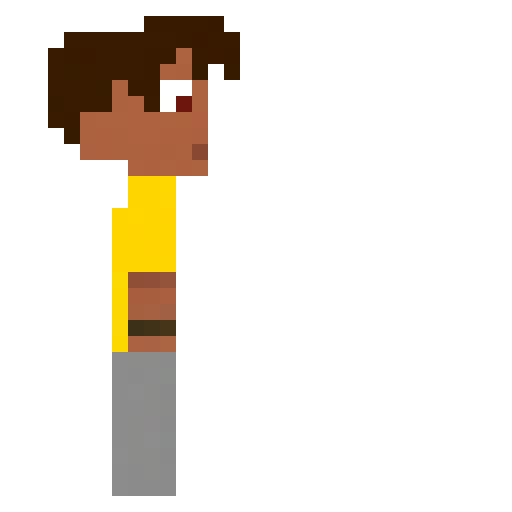
\includegraphics[width=1\linewidth]{figs/geminiPro/fix grande.png}
        \caption{\small Sprite do personagem Pablo em side view gerado pelo Gemini Pro}
        \label{fig:pixelLabPabloGeminiProSide}
    \end{subfigure}
    \begin{subfigure}{0.45\linewidth}
        \centering
        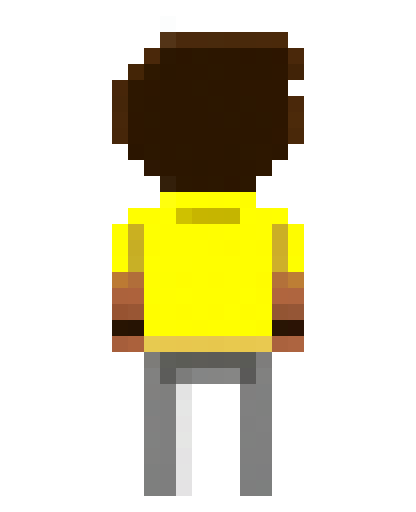
\includegraphics[width=0.8\linewidth]{figs/geminiPro/back_pixel_grande.png}
        \caption{\small Sprite do personagem Pablo de costas gerado pelo Gemini Pro}
        \label{fig:pixelLabPabloGeminiProCostas}
    \end{subfigure}
    \begin{subfigure}{0.45\linewidth}
        \centering
        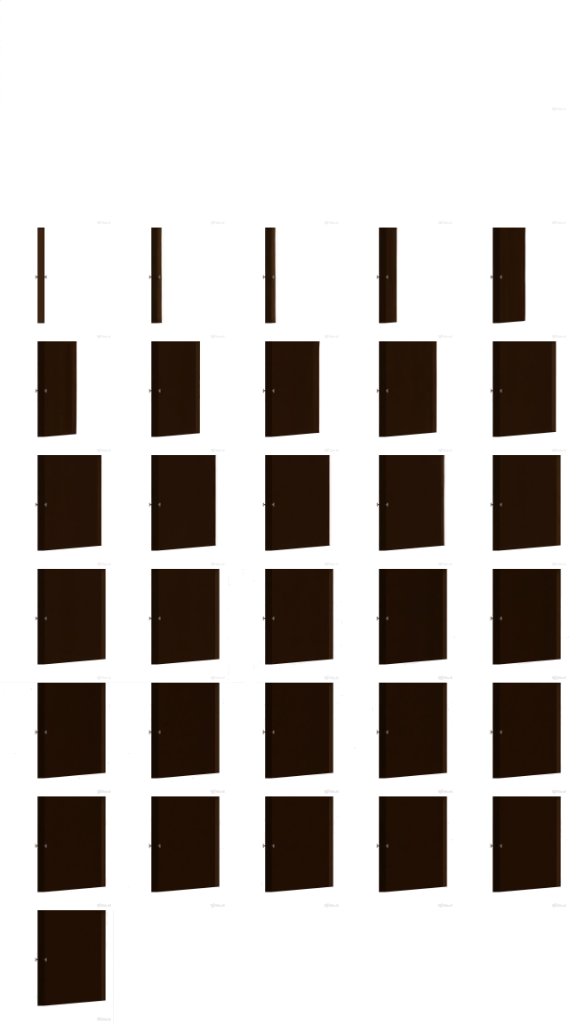
\includegraphics[width=1\linewidth]{figs/vidu/Pixilart/porta_sprite_sheet_pixel.png}
        \caption{\small Sprite sheet da porta abrindo gerado pelo Vidu}
        \label{fig:pixelLabPortaViduSideView}
    \end{subfigure}
    \begin{subfigure}{0.45\linewidth}
        \centering
        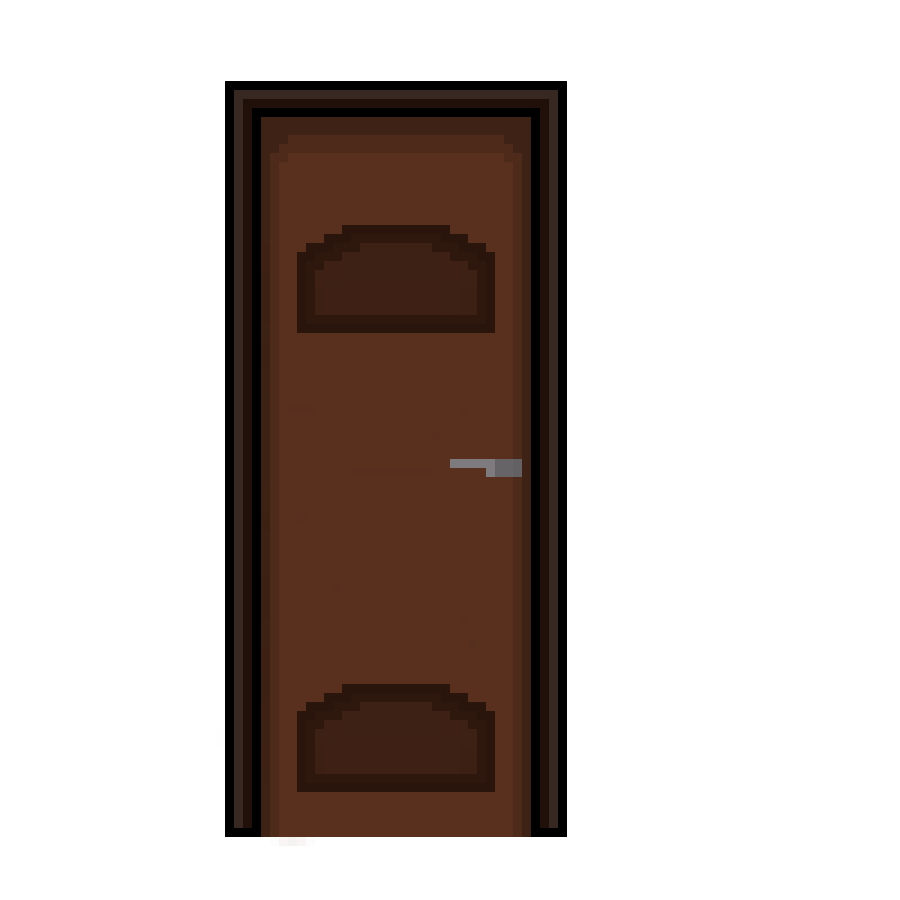
\includegraphics[width=1\linewidth]{figs/sprites/Porta front view.png}
        \caption{\small Sprite da porta em side view fechada}
        \label{fig:pixelLabPortaSideView}
    \end{subfigure}
    \legend{\small Fonte: Elaborada pela autora.}
\end{figure}

%   ------------------------------------------------------------------------
\FloatBarrier
\subsection{Ferramenta de rotação}
\label{s.pixelLab.rotacao}

A ferramenta de rotação possui dois formatos: o componente chamado quick rotate (rotação rápida, em inglês) mostrado na Figura \ref{fig:pixelLabQuickRotateTela} no Apêndice \ref{ap.telasIA}, no qual, após ser selecionado pelo usuário, gera a nova imagem de acordo com o quanto foi arrastado horizontalmente (para definir o ângulo da rotação) e verticalmente (para o ângulo da inclinação) desde o momento do clique do mouse até a sua soltura; e a seção rotate (rotação, em inglês), que abre uma tela com várias configurações para gerar o personagem rotacionado, como pode ser visto na Figura \ref{fig:pixelLabRotateTela} no Apêndice \ref{ap.telasIA}. 

De acordo com a documentação, a ferramenta é melhor em fazer rotações pequenas, de forma que o resultado de uma rotação pode ser usado como a imagem inicial a ser rotacionada. Nesse método, porém, os erros são acumulados a cada rotação. Enquanto isso, há também a possibilidade de apenas fazer a rotação maior para evitar o acúmulo de erros, apesar de ser mais complicado para a IA.

Os testes dessa funcionalidade específica visavam criar a imagem do Pablo em side view, a partir do sprite mostrado na Figura \ref{fig:Pablo}.

Durante as primeiras tentativas, os resultados (Figura \ref{fig:pixelLabRotacao1}) não geraram nenhuma rotação, apenas fazendo deformações no personagem. Porém, foi descoberto em testes posteriores que, para a geração de um bom resultado, o sprite deve estar centralizado no meio da tela, como pode ser visto na Figura \ref{fig:pixelLabRotCompara}.


\begin{figure}[htbp]
    \centering
    \caption{\small Comparação rotação 90 graus no Pixel Lab}
    \label{fig:pixelLabRotCompara}
    \begin{subfigure}{0.45\linewidth}
        \centering
        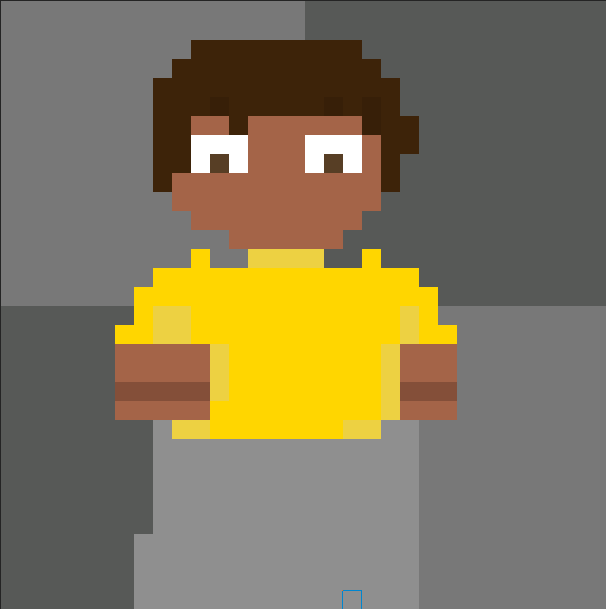
\includegraphics[width=0.5\linewidth]{figs/pixelLab/dia1/resultado rotacao 2.PNG}
        \caption{\small Resultado a partir do sprite inicialmente no canto esquerdo da tela}
        \label{fig:pixelLabRotComparaCanto}
    \end{subfigure}
    \begin{subfigure}{0.45\linewidth}
        \centering
        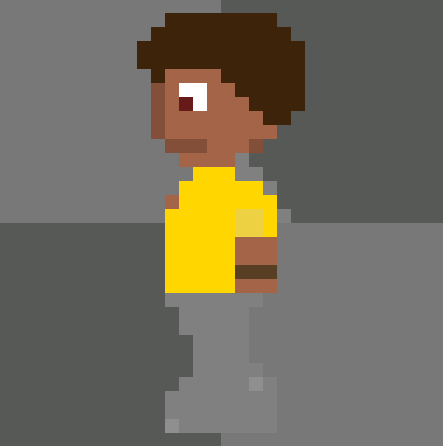
\includegraphics[width=0.5\linewidth]{figs/pixelLab/dia2/rot90res1.PNG}
        \caption{\small Resultado a partir do sprite inicialmente no centro da tela}
        \label{fig:pixelLabRotComparaCentro}
    \end{subfigure}

    \legend{\small Fonte: Elaborada pela autora, utilizando a ferramenta Pixel Lab.}
\end{figure}

Dessa forma, os testes prosseguiram posicionando a imagem corretamente, gerando rotações consistentes com o personagem e o estilo, porém com algumas deformações. Analisando os resultados, foi possível perceber que a ferramenta apresenta uma dificuldade na região onde ficaria o nariz, gerando essa parte com mais imperfeições. Além disso, foi notado que existe um processo para conseguir usar somente as cores da imagem de referência:
\begin{itemize}
    \item A imagem é gerada sem restrição nas cores (Figura \ref{fig:pixelLabProcesso1});
    \item A imagem é recriada com tons de cores similares aos da paleta do sprite original, não possuindo restrição no número de tonalidades (Figura \ref{fig:pixelLabProcesso2}); e
    \item O fundo é removido e cada uma das cores é igualada à mais semelhante da paleta original (Figura \ref{fig:pixelLabProcesso3}).
\end{itemize}

\begin{figure}[htbp]
    \centering
    \caption{\small Etapas do processamento da geração de imagem no Pixel Lab}
    \label{fig:pixelLabRotProcesso}
    \begin{subfigure}{0.32\linewidth}
        \centering
        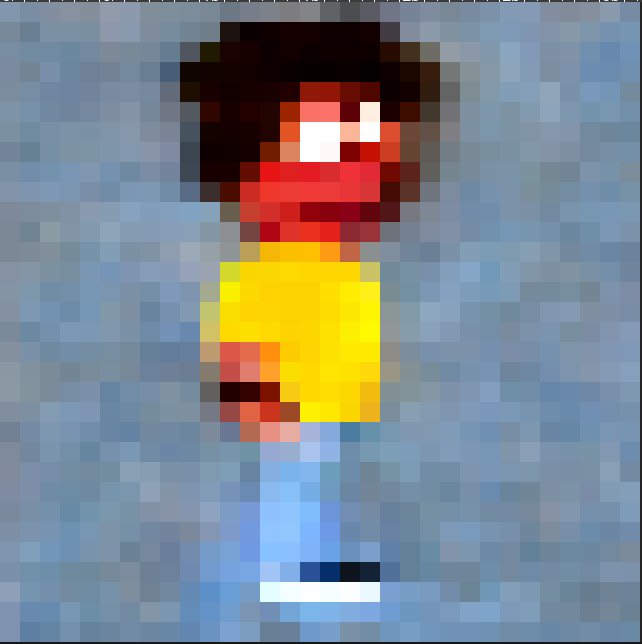
\includegraphics[width=1\linewidth]{figs/pixelLab/dia2/cores_tudo_estranha.PNG}
        \caption{\small Imagem da rotação no início do processamento}
        \label{fig:pixelLabProcesso1}
    \end{subfigure}
    \begin{subfigure}{0.32\linewidth}
        \centering
        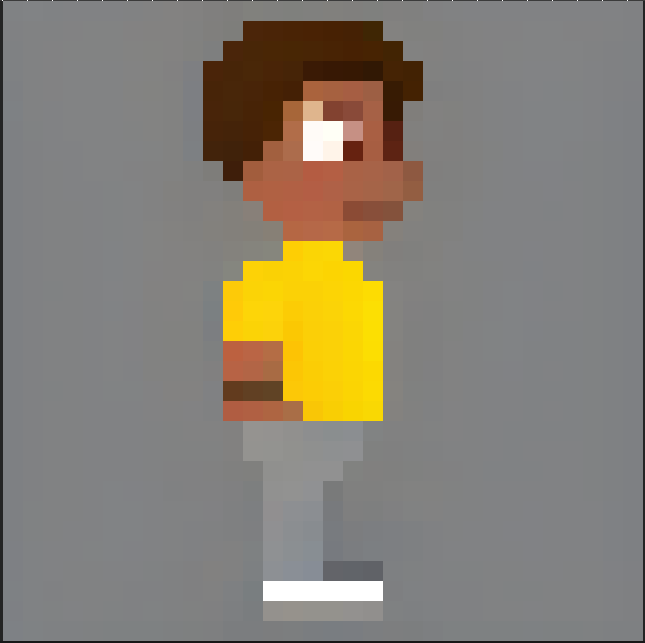
\includegraphics[width=1\linewidth]{figs/pixelLab/dia2/perna_antes_de_sumir.PNG}
        \caption{\small Imagem da rotação no meio do processamento, com cores mais parecidas às do sprite original, porém com mais tons}
        \label{fig:pixelLabProcesso2}
    \end{subfigure}
    \begin{subfigure}{0.32\linewidth}
        \centering
        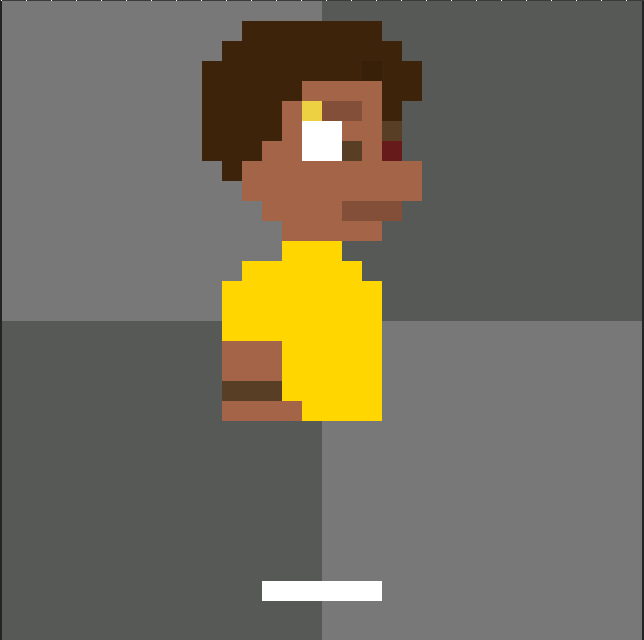
\includegraphics[width=1\linewidth]{figs/pixelLab/dia2/demonstrar_perna_sumindo.PNG}
        \caption{\small Imagem da rotação após o processamento, com cores igualadas ao do sprite original, porém removendo a perna}
        \label{fig:pixelLabProcesso3}
    \end{subfigure}

    \legend{\small Fonte: Elaborada pela autora, utilizando a ferramenta Pixel Lab.}
\end{figure}

Esse processo faz com que nem todas as características do personagem possuam a cor correta, além de muitas vezes causar o desaparecimento da calça por reconhecê-la como parte do fundo, já que as cores são semelhantes. Esses detalhes são mostrados na Figura \ref{fig:pixelLabRotComparaCor}. A demonstração completa dos testes é encontrada nas Figuras \ref{fig:pixelLabRotacao2} a \ref{fig:pixelLabRotacao4}.

\begin{figure}[htbp]
    \centering
    \caption{\small Comparação de cores entre o sprite original e o resultado gerado no Pixel Lab}
    \label{fig:pixelLabRotComparaCor}
    \begin{subfigure}{0.45\linewidth}
        \centering
        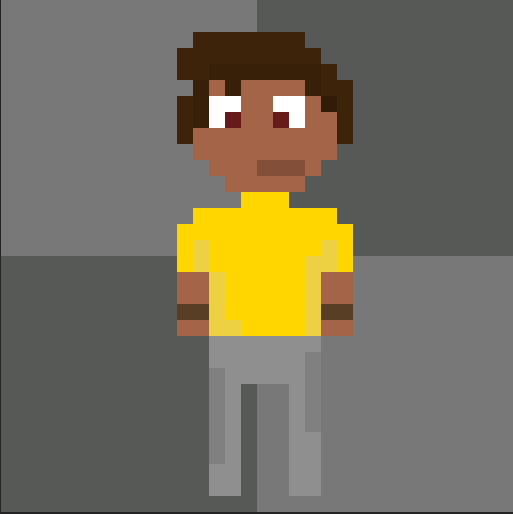
\includegraphics[width=1\linewidth]{figs/pixelLab/dia2/sprite_centro.PNG}
        \caption{\small Imagem original com olho castanho escuro e calça completa}
        \label{fig:pixelLabRotComparaCorA}
    \end{subfigure}
    \begin{subfigure}{0.45\linewidth}
        \centering
        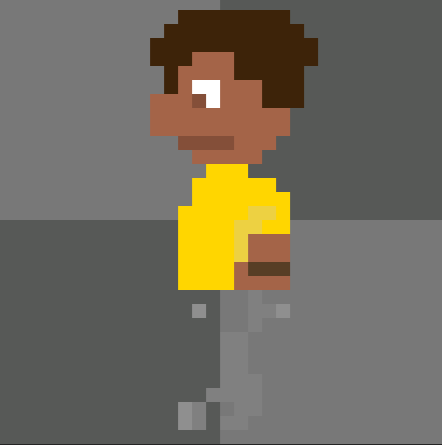
\includegraphics[width=1\linewidth]{figs/pixelLab/dia2/rot90res2.PNG}
        \caption{\small Resultado com olho castanho claro e parte da calça faltando}
        \label{fig:pixelLabRotComparaCorB}
    \end{subfigure}

    \legend{\small Fonte: Elaborada pela autora, utilizando a ferramenta Pixel Lab.}
\end{figure}

Na bateria seguinte de testes, foram realizados ajustes finos em algumas das imagens geradas de 45°, com o objetivo de gerar novamente o personagem em 90°, em uma tentativa de contornar o problema dos erros cumulativos. Como a ferramenta possui um editor integrado, é extremamente fácil e eficiente corrigir erros, diferente do que aconteceu em outras ferramentas. As edições feitas podem ser consultadas na Figura \ref{fig:pixelLabAjusteFino1} abaixo e na Figura \ref{fig:pixelLabAjusteFino2} no Apêndice \ref{ap.telasIA}.

\begin{figure}[htbp]
    \centering
    \caption{\small Ajuste fino no resultado da rotação de 45 graus no Pixel Lab}
    \label{fig:pixelLabAjusteFino1}
    \begin{subfigure}{0.45\linewidth}
        \centering
        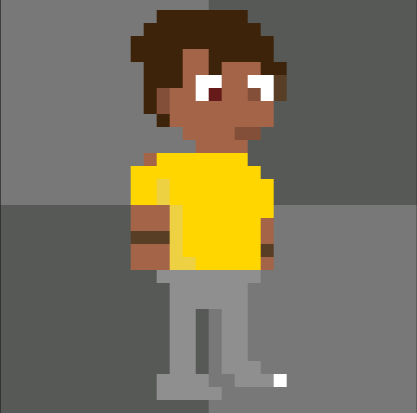
\includegraphics[width=1\linewidth]{figs/pixelLab/dia2/rot45res4.PNG}
        \caption{\small Antes da edição}
        \label{fig:pixelLabAjusteFino1a}
    \end{subfigure}
    \begin{subfigure}{0.45\linewidth}
        \centering
        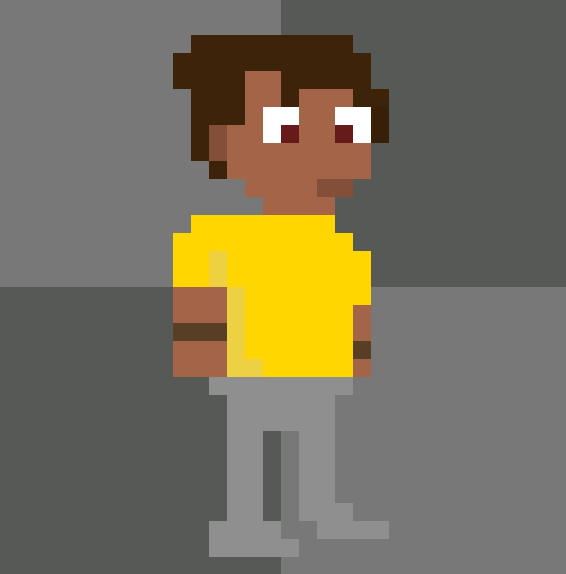
\includegraphics[width=1\linewidth]{figs/pixelLab/dia2/fix_teste_4.PNG}
        \caption{\small Após edição}
        \label{fig:pixelLabAjusteFino1b}
    \end{subfigure}

    \legend{\small Fonte: Elaborada pela autora, utilizando a ferramenta Pixel Lab.}
\end{figure}

Após esse ajuste, mais testes foram feitos, porém os resultados gerados (Figuras \ref{fig:pixelLabRotacao6} a \ref{fig:pixelLabRotacao9} no Apêndice \ref{ap.telasIA}) não mostraram nenhuma melhora significativa, aparentando possuir mais deformações e imprecisões do que anteriormente. Isso pode ser melhor notado na Figura \ref{fig:pixelComparaAjuste}.

\begin{figure}[htbp]
    \centering
    \caption{\small Comparação de resultados antes e depois do ajuste fino}
    \label{fig:pixelComparaAjuste}
    \begin{subfigure}{0.45\linewidth}
        \centering
        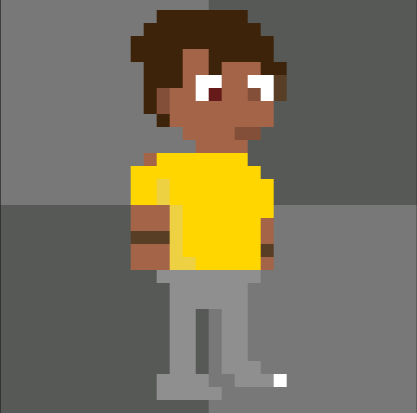
\includegraphics[width=1\linewidth]{figs/pixelLab/dia2/rot45res4.PNG}
        \caption{\small Resultado gerado a partir da imagem sem o ajuste fino, com uma deformação na região do nariz e boca e erros e pequenos erros na proporção do corpo}
        \label{fig:pixelComparaAjusteAntes}
    \end{subfigure}
    \begin{subfigure}{0.45\linewidth}
        \centering
        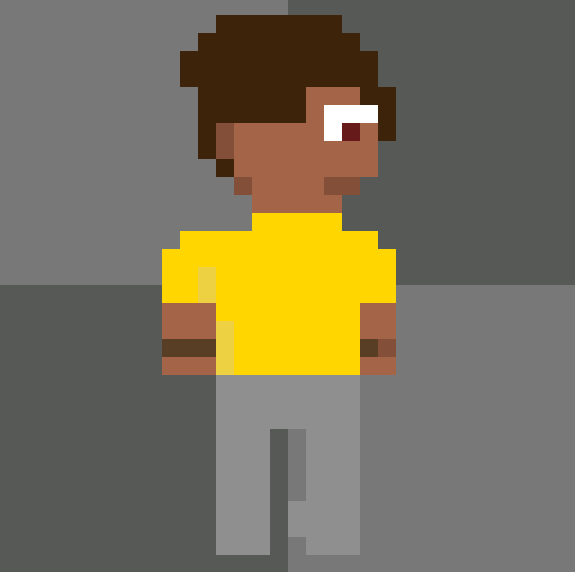
\includegraphics[width=1\linewidth]{figs/pixelLab/dia2/rot45fix3res2.PNG}
        \caption{\small Resultado gerado a partir da imagem com o ajuste fino, onde apenas a cabeça do sprite gerado aparenta estar rotacionada e com um deformação no olho}
        \label{fig:pixelComparaAjusteDepois}
    \end{subfigure}

    \legend{\small Fonte: Elaborada pela autora, utilizando a ferramenta Pixel Lab.}
\end{figure}

Considerando a falha na abordagem anterior, uma nova estratégia foi montada considerando uma das opções de customização que a ferramenta rotate oferece: init image (imagem de inicialização, em inglês). Essa funcionalidade permite ao usuário indicar uma imagem para guiar a IA em como deve ficar o resultado final, tendo uma variável associada chamada init image strength (força da imagem de inicialização, em inglês) para indicar o quanto essa inicialização deve ser utilizada. 

Na primeira instância, o melhor resultado gerado do personagem em side view na ferramenta é usado como imagem de inicialização, como pode ser visto na Figura \ref{fig:pixelLabRotInit} no Apêndice \ref{ap.telasIA}.

Os resultados gerados (Figura \ref{fig:pixelLabRotacao10} no Apêndice \ref{ap.telasIA}) apresentaram uma melhor performance comparada aos sprites gerados sem nenhuma imagem de inicialização, porém demonstraram erros na região da calça, o que também pode ser visto na imagem de inicialização, apesar de com menos intensidade. Devido a esse fator, foi feita uma edição na init image, que pode ser vista na Figura \ref{fig:pixelLabAjusteFino3}.

\begin{figure}[htbp]
    \centering
    \caption{\small Edição no resultado da rotação de 90 graus no Pixel Lab}
    \label{fig:pixelLabAjusteFino3}
    \begin{subfigure}{0.45\linewidth}
        \centering
        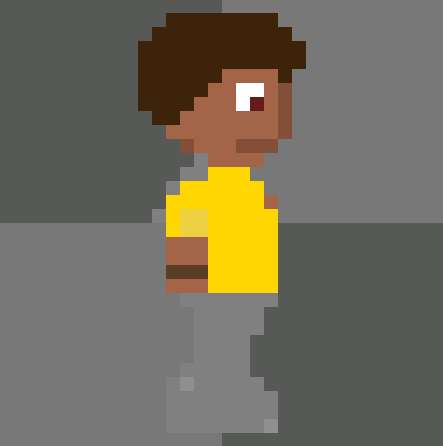
\includegraphics[width=1\linewidth]{figs/pixelLab/dia2/init.PNG}
        \caption{\small Antes da edição}
        \label{fig:pixelLabAjusteFino3a}
    \end{subfigure}
    \begin{subfigure}{0.45\linewidth}
        \centering
        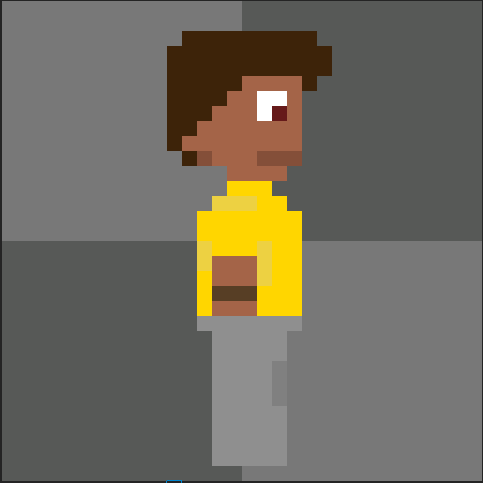
\includegraphics[width=1\linewidth]{figs/pixelLab/dia2/fix_init_1.PNG}
        \caption{\small Após edição}
        \label{fig:pixelLabAjusteFino3b}
    \end{subfigure}

    \legend{\small Fonte: Elaborada pela autora, utilizando a ferramenta Pixel Lab.}
\end{figure}

Analisando as imagens geradas (Figura \ref{fig:pixelLabRotacao11} no Apêndice \ref{ap.telasIA}) ainda não foi encontrado nenhum resultado satisfatório, com todos os sprites gerados sem as pernas.

Reavaliando todos os resultados, apesar da ferramenta quase ter gerado resultados satisfatórios, nenhum dos sprites alcança os padrões de qualidade para sua aplicação no jogo. Porém, a Figura \ref{fig:pixelLabAjusteFino2c} no Apêndice \ref{ap.telasIA} e a Figura  \ref{fig:pixelLabAjusteFino3b} foram usadas como referência para fornecer um contexto maior do personagem nas ferramentas ChatGPT (detalhada na Seção \ref{s.chatGPT}) e GeminiPro (detalhada na Seção \ref{s.ferramentaB}).

A análise da funcionalidade de rotação indica que, embora a ferramenta não elimine a necessidade de intervenção manual, ela otimiza o processo de criação. Os resultados, embora exijam edições e ajustes finos para atingir a qualidade desejada, fornecem uma base com alta consistência e fidelidade que auxilia na produção dos sprites do personagem.


%   ------------------------------------------------------------------------
\FloatBarrier
\subsection{Ferramenta de animação para animação}
\label{s.pixelLab.animacao}

A ferramenta de animation to animation (animação para animação, em inglês) utiliza o sprite de uma pessoa e uma animação qualquer como referências para animar o movimento desse personagem. A funcionalidade pode gerar até 15 frames e também usa uma descrição do personagem a ser animado e da ação a ser feita, com opções de customização do contorno e shading (sombreamento, em inglês) que o resultado final deve ter. A  funcionalidade de limitação de cores considera a paleta do primeiro frame da animação de base, e não do sprite de referência. Existem também duas variáveis que influenciam a geração: AI freedom (liberdade da IA, em inglês), que determina o quanto a IA deve imitar a animação de referência; e guidance weight (peso da orientação, em inglês), que indica o quanto a descrição influencia no resultado.

O objetivo da primeira bateria de testes dessa funcionalidade foi gerar uma animação do personagem Pablo andando, utilizando como base o sprite sheet gerado pela ferramenta God Mode AI (Figura \ref{fig:pixelLabSpriteSheetGodModeAI}). Antes de ser usada como referência, a imagem gerada pela ferramenta Gemini Pro (detalhada na Seção \ref{s.ferramentaB}) do personagem Pablo em side view (Figura \ref{fig:pixelLabPabloGeminiProSide}) passou por ajustes finos, como pode ser visto na Figura \ref{fig:pixelLabAniSideViewSprite1}. É importante notar que este sprite representa uma versão intermediária do resultado final da edição. Análises posteriores levaram a um refinamento adicional, cujo processo é detalhado na Seção \ref{s.pixelLab.edicao}, resultando na versão final utilizada no jogo.

\begin{figure}[htbp]
    \centering
    \caption{\small Sprite do personagem em side view após ajuste fino}
    \label{fig:pixelLabAniSideViewSprite1}
    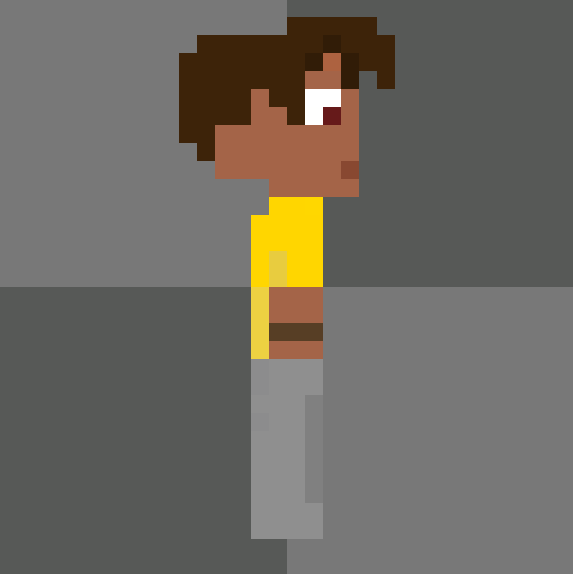
\includegraphics[width=0.4\linewidth]{figs/pixelLab/dia3/fixGrande.PNG}
    \legend{\small Fonte: Elaborada pela autora.}
\end{figure}

Durante o teste inicial, a imagem corrigida e a animação citada anteriormente são colocadas como referência, enquanto é utilizado um prompt simples que descreve as roupas usadas pelo personagem, como pode ser verificado na Figura \ref{fig:pixelLabAniTela}.


\begin{figure}[htbp]
    \centering
    \caption{\small Tela da geração de animação no Pixel Lab}
    \label{fig:pixelLabAniTela}
    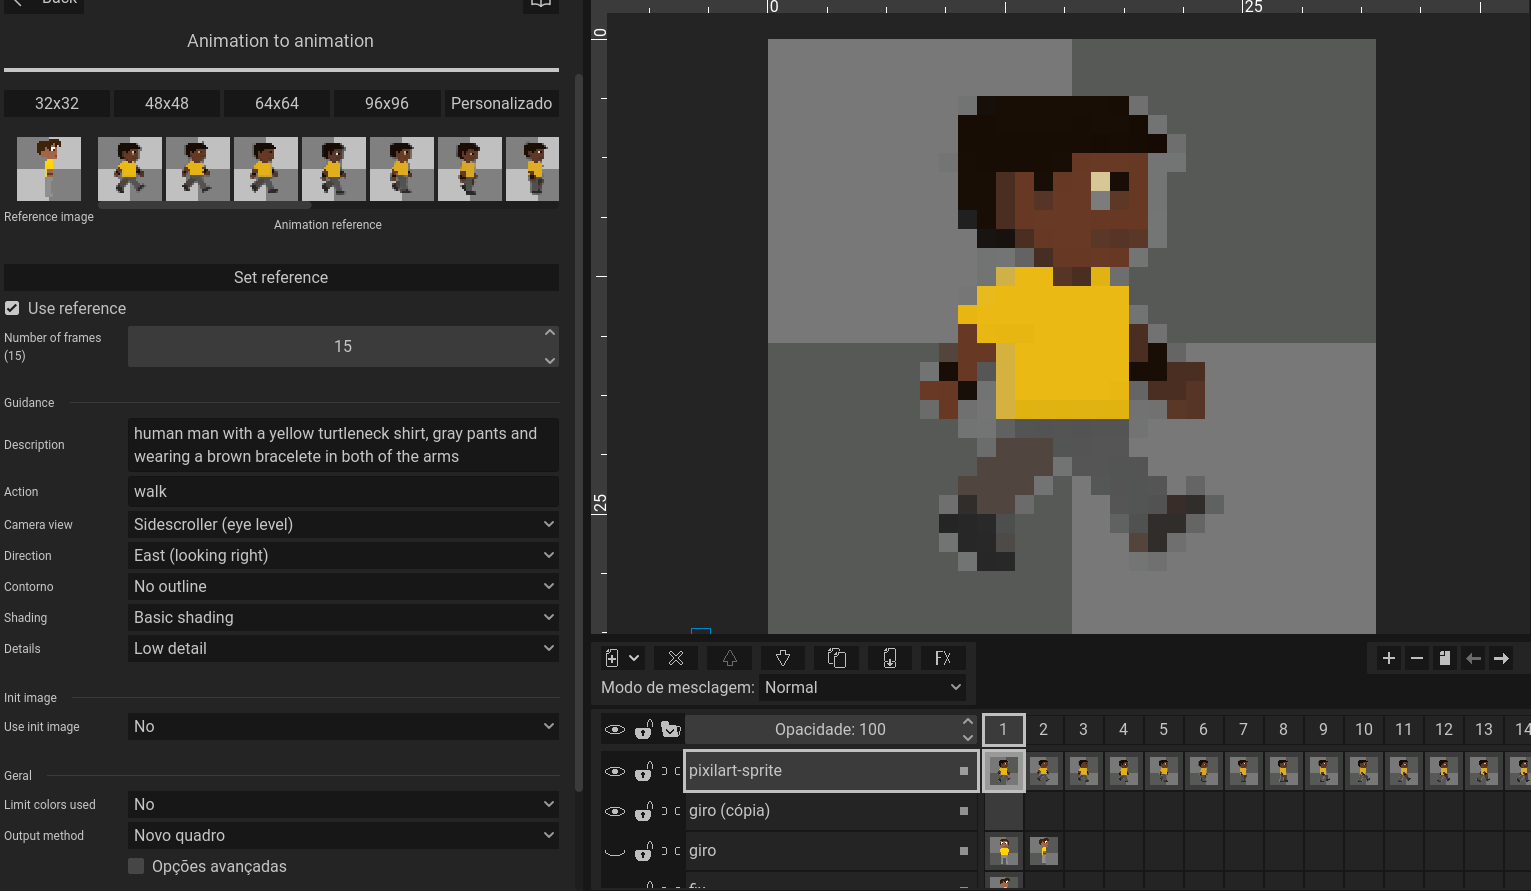
\includegraphics[width=1\linewidth]{figs/pixelLab/dia3/tela_animacao.PNG}
    \legend{\small Fonte: Elaborada pela autora.}
\end{figure}

O resultado gerado\footnote{\url{https://drive.google.com/file/d/1TYecwF1D5EqbKaJIOJle_iZbkVOuWsux/view?usp=sharing}} foi insatisfatório, apresentando uma aparência diferente do personagem de referência, além de não possuir o mesmo estilo de pixel art, como pode ser visto na Figura \ref{fig:pixelLabAniResRuim}.

\begin{figure}[htbp]
    \centering
    \caption{\small Quadro da animação gerada no Pixel Lab}
    \label{fig:pixelLabAniResRuim}
    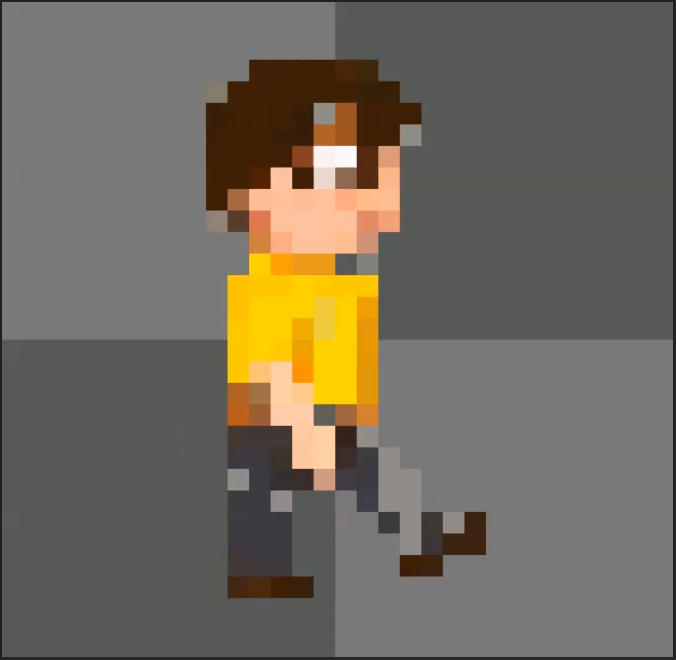
\includegraphics[width=0.4\linewidth]{figs/pixelLab/dia3/print1.PNG}
    \legend{\small Fonte: Elaborada pela autora.}
\end{figure}

Levando em conta esse erro, em testes posteriores foi adicionada a descrição da aparência do personagem no prompt como pode ser verificado na Figura \ref{fig:pixelLabAniPrompt}. Durante cada uma das interações, algumas palavras do prompt e as configurações de sombreamento são mudadas, visando obter um resultado mais consistente com o sprite de referência. As tentativas completas podem ser consultadas nas Figuras \ref{fig:pixelLabAnimacao1} a \ref{fig:pixelLabAnimacao6} do Apêndice \ref{ap.telasIA}. 

\begin{figure}[htbp]
    \centering
    \caption{\small Prompt com a descrição da aparência}
    \label{fig:pixelLabAniPrompt}
    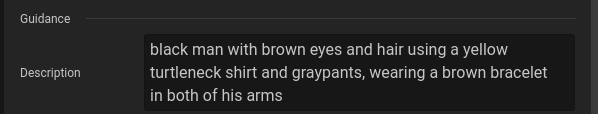
\includegraphics[width=0.7\linewidth]{figs/pixelLab/dia3/prompt.PNG}
    \legend{\small Fonte: Elaborada pela autora.}
\end{figure}

A geração de uma animação possui o mesmo processo da geração de imagem, o que faz sentido considerando que um vídeo é formado por várias figuras (quadros). 

Durante um dos testes, ocorreu algo inesperado: nenhuma animação foi gerada. Investigando mais a fundo, foi descoberto que, na última etapa do processamento, onde o fundo deveria ser removido, o sprite inteiro foi deletado. Esse erro não se repetiu em mais nenhum outro teste. Abaixo se encontram as Figuras \ref{fig:pixelLabAniPromptFalha} e \ref{fig:pixelLabAniTelaFalha} mostrando o prompt usado e o resultado gerado na interação falha.


\begin{figure}[htbp]
    \centering
    \caption{\small Prompt que gerou a falha no Pixel Lab}
    \label{fig:pixelLabAniPromptFalha}
    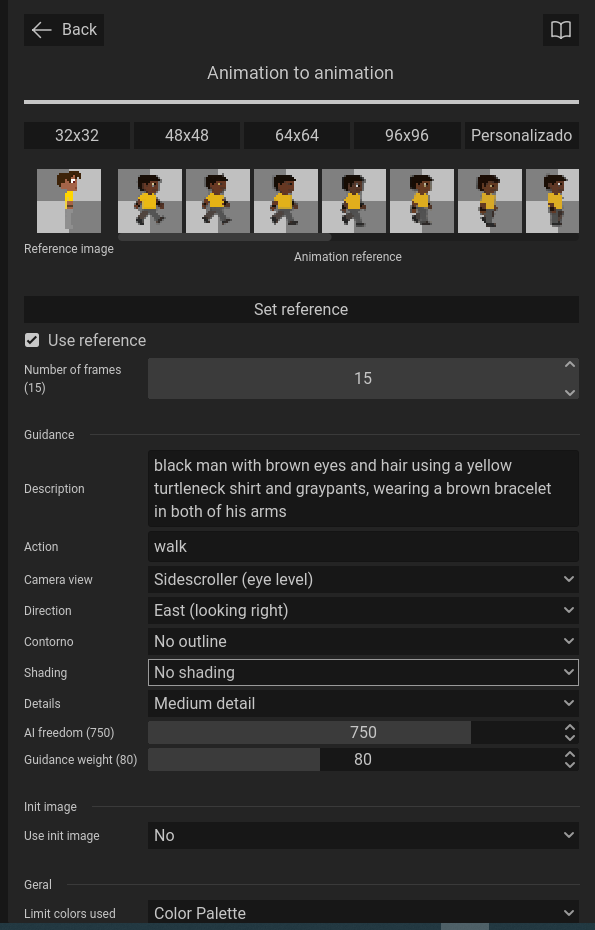
\includegraphics[width=0.53\linewidth]{figs/pixelLab/dia3/tela_3.PNG}
    \legend{\small Fonte: Elaborada pela autora.}
\end{figure}

\begin{figure}[htbp]
    \centering
    \caption{\small Quadros vazios após a geração no Pixel Lab}
    \label{fig:pixelLabAniTelaFalha}
    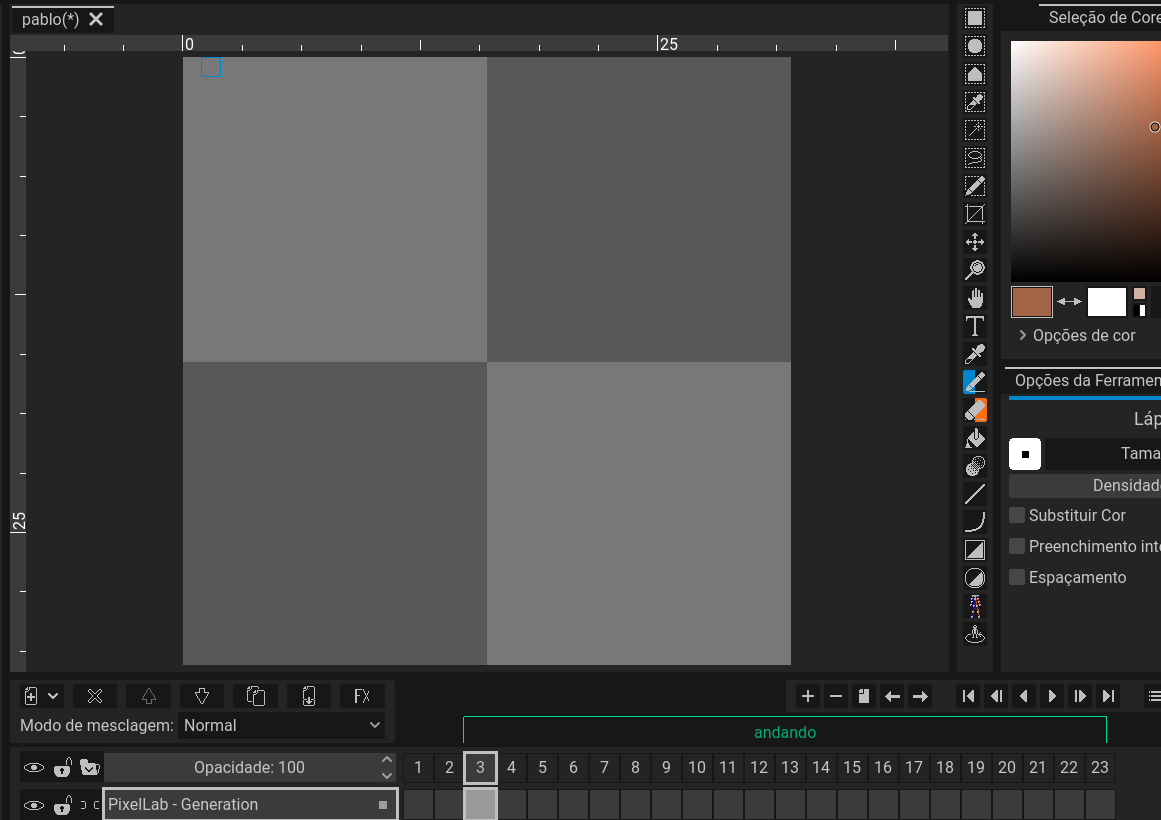
\includegraphics[width=0.7\linewidth]{figs/pixelLab/dia3/falha3.PNG}
    \legend{\small Fonte: Elaborada pela autora.}
\end{figure}

Analisando os resultados, nenhum deles manteve o formato da silhueta original, os tons de cores ficaram levemente distintos do personagem a ser animado e possuíam falhas de pixels que tornavam as características do rosto menos reconhecíveis. Foi possível notar que o tamanho e a forma do sprite da animação de referência influenciaram as imagens geradas, o que pode ser observado mais atentamente na Figura \ref{fig:pixelLabAnimaCompara}. Investigando mais a fundo, isso acontece por causa do funcionamento da funcionalidade animação para animação, que cria o esqueleto da animação de referência, e usa a movimentação que o esqueleto apresentou para criar uma nova animação. O esqueleto da animação de base mantém o formato e o tamanho da mesma, e o resultado final é gerado por cima desse esqueleto, utilizando as características deste.

\begin{figure}[htbp]
    \centering
    \caption{\small Comparação do sprite original com os frames da animação de base e da gerada no Pixel Lab}
    \label{fig:pixelLabAnimaCompara}

    \begin{subfigure}{0.32\linewidth}
        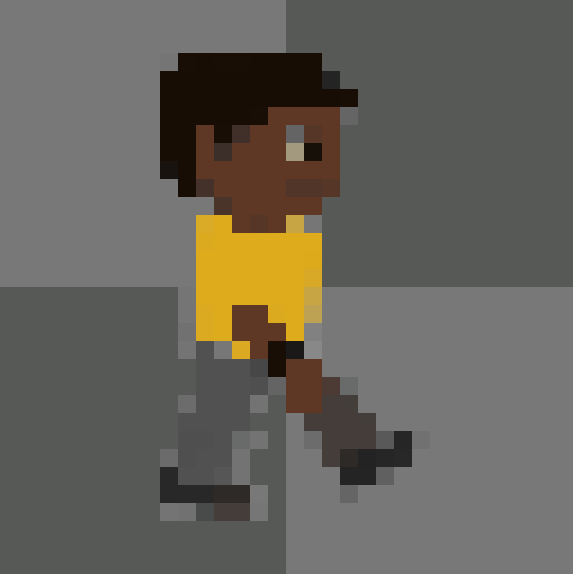
\includegraphics[width=0.9\linewidth]{figs/pixelLab/dia3/print0.PNG}
        \caption{\small Frames da animação de referência}
        \label{fig:pixelLabAnimaComparaAni}
    \end{subfigure}
    \begin{subfigure}{0.32\linewidth}
        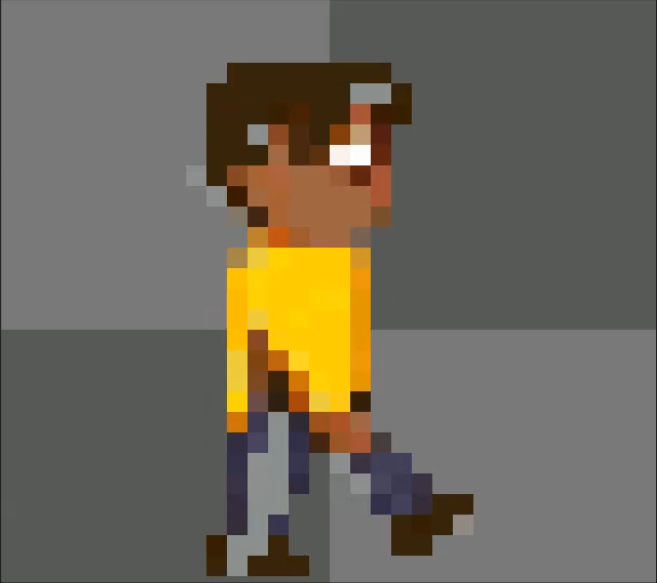
\includegraphics[width=1\linewidth]{figs/pixelLab/dia3/print4.PNG}
        \caption{\small Frame da animação gerada }
        \label{fig:pixelLabAnimaComparaGera}
    \end{subfigure}
    \begin{subfigure}{0.32\linewidth}
        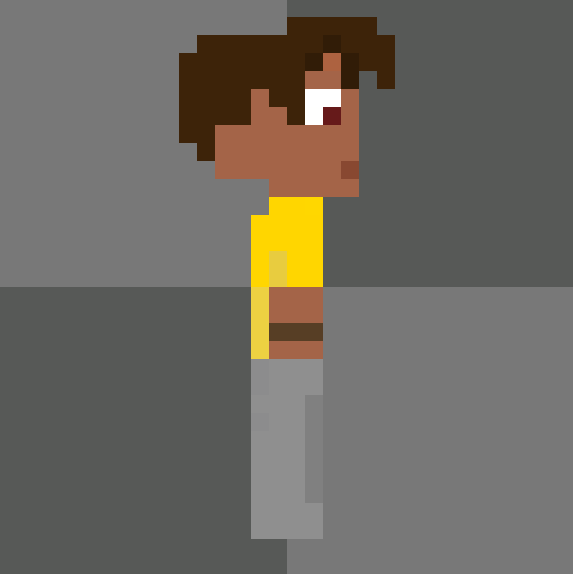
\includegraphics[width=0.9\linewidth]{figs/pixelLab/dia3/fixGrande.PNG}
        \caption{\small Sprite original em side view }
        \label{fig:pixelLabAnimaComparaSprite}
    \end{subfigure}
    \legend{\small Fonte: Elaborada pela autora, utilizando a ferramenta Pixel Lab.}
\end{figure}


A análise mostra que usar a ferramenta com uma animação que não é consistente com o sprite em tamanho e formato não gera resultados satisfatórios que possam ser aplicados em um jogo. Considerando esse fator, posteriormente foi realizada uma segunda bateria de testes, utilizando para a geração da nova animação o sprite sheet do vídeo do personagem Pablo andando gerado pela ferramenta Gemini Pro (Figura \ref{fig:pixelLabSpriteSheetGeminiPro}), que possui características extremamente próximas ao sprite original, porém apresenta pequenos erros. Além disso, como imagem de referência será usada a versão final do ajuste fino do sprite do personagem Pablo em side view gerado pelo Gemini Pro (Figura \ref{fig:pixelLabAniSideViewSprite2}).

\begin{figure}[htbp]
    \centering
    \caption{\small Quadro da animação gerada no Pixel Lab}
    \label{fig:pixelLabAniSideViewSprite2}
    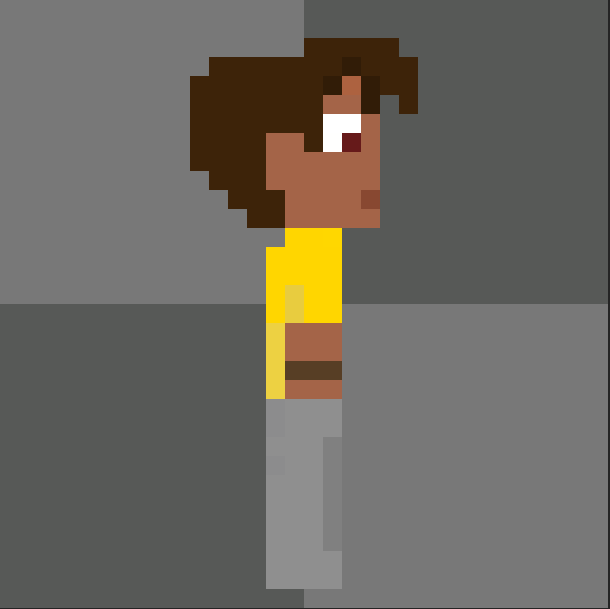
\includegraphics[width=0.4\linewidth]{figs/pixelLab/dia3/fix_oficial_fundo_igual.PNG}
    \legend{\small Fonte: Elaborada pela autora.}
\end{figure}

Os resultados\footnote{\url{https://drive.google.com/drive/folders/1xmE-wpvT9xLguyX2izbWv2Xn0glh84IZ?usp=sharing}} gerados obtiveram uma alta consistência, porém a qualidade deles foi menor do que a da animação de referência, com tons de cores diferentes do sprite original e erros nos pixels, porém possuindo o formato mais preciso da mão, como pode ser visto na Figura \ref{fig:pixelLabAnimaComparaGemini}. A interação completa pode ser consultada nas Figuras \ref{fig:pixelLabAnimacao7} e \ref{fig:pixelLabAnimacao8} do Apêndice \ref{ap.telasIA}. 

\begin{figure}[htbp]
    \centering
    \caption{\small Comparação do sprite de referência com os frames da animação de base e da gerada no Pixel Lab}
    \label{fig:pixelLabAnimaComparaGemini}

    \begin{subfigure}{0.32\linewidth}
        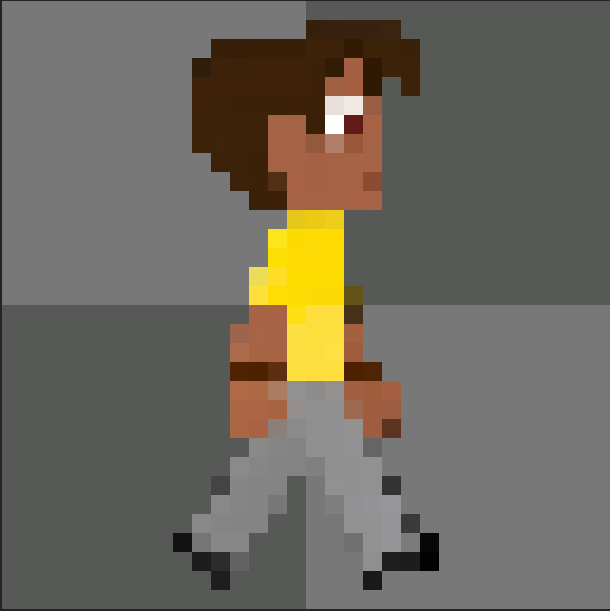
\includegraphics[width=1\linewidth]{figs/pixelLab/dia4/print0.PNG}
        \caption{\small Frame da animação de referência, com cores mais precisas e dedão na mão visível}
        \label{fig:pixelLabAnimaComparaGeminiAni}
    \end{subfigure}
    \begin{subfigure}{0.32\linewidth}
        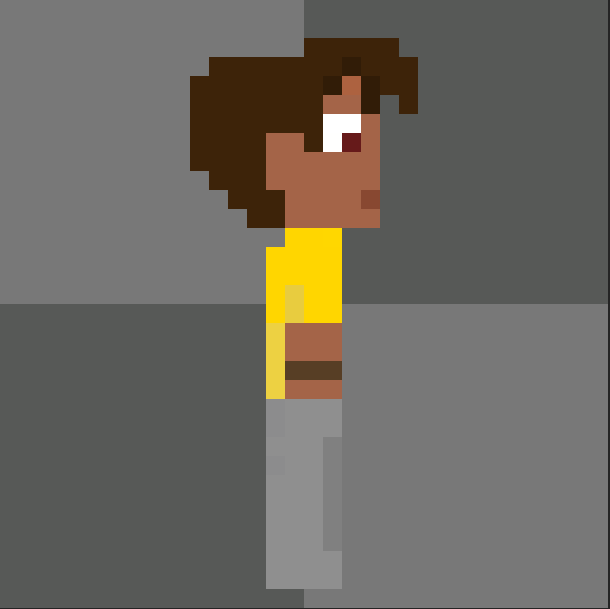
\includegraphics[width=1\linewidth]{figs/pixelLab/dia3/fix_oficial_fundo_igual.PNG}
        \caption{\small Sprite de referência em side view, sem dedão visível na mão}
        \label{fig:pixelLabAnimaComparaGeminiSprite}
    \end{subfigure}
    \begin{subfigure}{0.32\linewidth}
        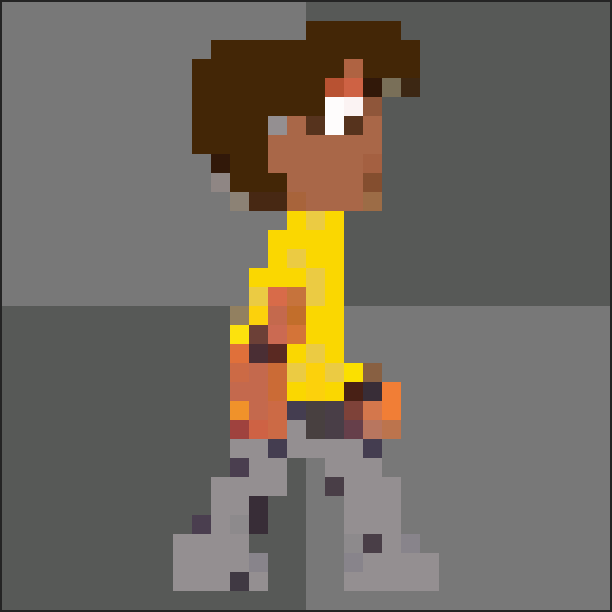
\includegraphics[width=1\linewidth]{figs/pixelLab/dia4/print1.PNG}
        \caption{\small Frame da animação gerada, com cores menos precisas e sem dedão na mão}
        \label{fig:pixelLabAnimaComparaGeminiGera}
    \end{subfigure}
    \legend{\small Fonte: Elaborada pela autora, utilizando a ferramenta Pixel Lab.}
\end{figure}

Nos testes posteriores, além de se utilizar a opção de limitar as cores da animação gerada de acordo com a paleta do primeiro frame, o mesmo foi editado para ter as cores exatas do sprite original. O objetivo era testar a capacidade da ferramenta na geração da animação, sem buscar apenas produzir uma animação melhor pela edição manual. Como a animação mostrada parcialmente na Figura \ref{fig:pixelLabAnimaComparaGeminiGera}, apesar de ter tons de cores diferentes, possui um formato mais preciso, ela também foi utilizada como referência após a do sprite original como primeiro quadro. 

Os resultados\footnote{\url{https://drive.google.com/drive/folders/1YHiklOXkW1FhYC_fBS00c21wt8fMNiIq?usp=drive_link}} obtiveram uma queda na qualidade, com as cores sendo utilizadas de maneira imprecisa e possuindo ainda mais erros nos pixels, como pode ser visto na Figura \ref{fig:pixelLabAnimaComparaGemini2}. Interações completas podem ser consultadas nas Figuras \ref{fig:pixelLabAnimacao9} a \ref{fig:pixelLabAnimacao11} no Apêndice \ref{ap.telasIA}. Investigando mais a fundo, é descoberto que esse declínio provavelmente foi causado pelo fato de que o sprite original não possui tons suficientes para trazer um efeito de profundidade na região das pernas e dos braços, fazendo a IA aplicar cores totalmente diferentes em regiões que precisam ter essa diferença.

\begin{figure}[htbp]
    \centering
    \caption{\small Comparação do sprite de referência com os frames das animações geradas no Pixel Lab}
    \label{fig:pixelLabAnimaComparaGemini2}

    \begin{subfigure}{0.32\linewidth}
        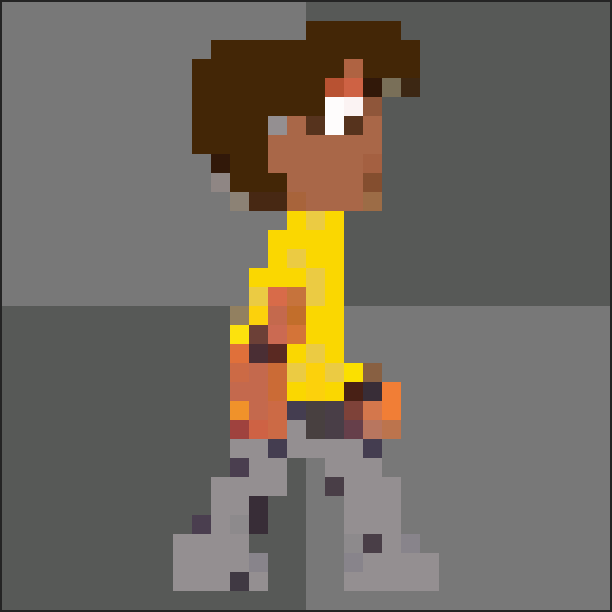
\includegraphics[width=1\linewidth]{figs/pixelLab/dia4/print1.PNG}
        \caption{\small Frame da animação gerada sem limitar as cores para apenas as mesmas do sprite de referência}
        \label{fig:pixelLabAnimaComparaGeminiAni2}
    \end{subfigure}
    \begin{subfigure}{0.32\linewidth}
        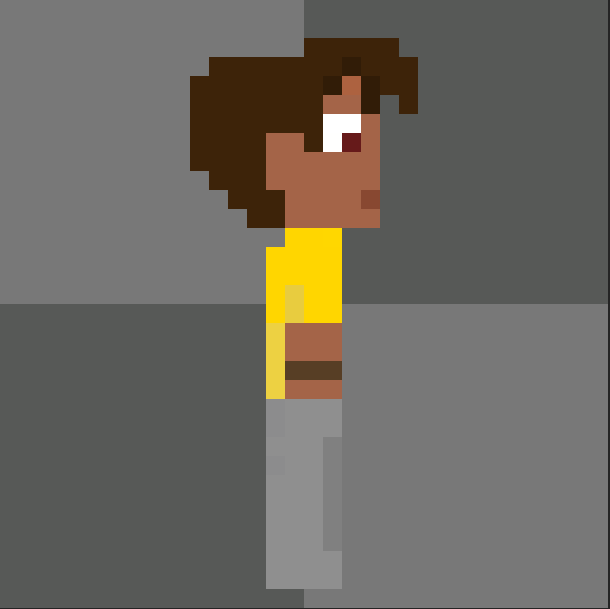
\includegraphics[width=1\linewidth]{figs/pixelLab/dia3/fix_oficial_fundo_igual.PNG}
        \caption{\small Sprite de referência em side view}
        \label{fig:pixelLabAnimaComparaGeminiSprite2}
    \end{subfigure}
    \begin{subfigure}{0.32\linewidth}
        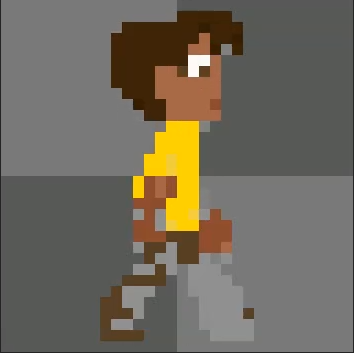
\includegraphics[width=1\linewidth]{figs/pixelLab/dia4/print6.PNG}
        \caption{\small Frame da animação gerada limitando as cores para apenas as mesmas do sprite de referência}
        \label{fig:pixelLabAnimaComparaGeminiGera2}
    \end{subfigure}
    \legend{\small Fonte: Elaborada pela autora, utilizando a ferramenta Pixel Lab.}
\end{figure}

Para explorar os limites da ferramenta, foi conduzido um último teste. O objetivo era verificar se essa funcionalidade também poderia ser utilizada para gerar uma animação de rotação completa, uma tarefa normalmente designada à ferramenta de rotação. 

Para isso, foi criada manualmente uma animação de pseudo-rotação utilizando os sprites já existentes do personagem Pablo (visão frontal, lateral, de costas e lateral espelhada), cada um ocupando um quadro para simular um giro de 360 graus. Esta animação serviu como referência de movimento. Como sprite de referência, foi utilizada a personagem Luz, que possui um corpo com proporções e tamanho significativamente diferentes. Naquele momento, ainda não havia sido compreendido totalmente que a animação gerada seguia o formato da animação de referência e não do sprite.

O resultado\footnote{\url{https://drive.google.com/file/d/1NEfmTRU46067ueFgWvvhpd1MQBiyhP1H/view?usp=sharing}} gerado foi completamente insatisfatório, produzindo uma animação completamente deformada que tentava aplicar as proporções maiores do personagem Pablo ao corpo menor da personagem Luz. Este experimento serviu como confirmação definitiva da teoria levantada nos testes anteriores: a ferramenta prioriza a estrutura geométrica e as proporções do esqueleto da animação de referência, em vez de seguir o formato do sprite de referência. A inconsistência dimensional entre os dois inputs leva inevitavelmente a um resultado de baixa precisão, como pode ser visto na Figura \ref{fig:pixelLabAnimaComparaRodarSprite}.

\begin{figure}[htbp]
    \centering
    \caption{\small Comparação do sprite original com os frames da animação gerada no Pixel Lab}
    \label{fig:pixelLabAnimaComparaRodar}

    \begin{subfigure}{0.32\linewidth}
        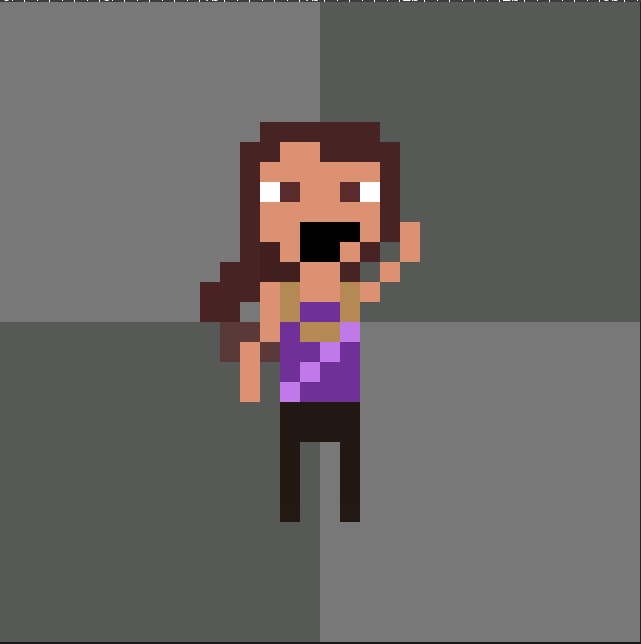
\includegraphics[width=1\linewidth]{figs/pixelLab/dia4/irma.PNG}
        \caption{\small Sprite original}
        \label{fig:pixelLabAnimaComparaRodarSprite}
    \end{subfigure}
    \begin{subfigure}{0.32\linewidth}
        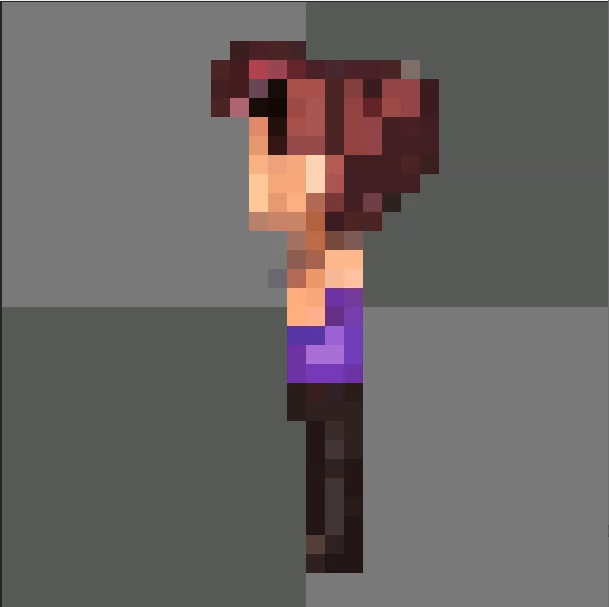
\includegraphics[width=1\linewidth]{figs/pixelLab/dia4/printA.PNG}
        \caption{\small Frame 1 da animação gerada }
        \label{fig:pixelLabAnimaComparaRodarFrame1}
    \end{subfigure}
    \begin{subfigure}{0.32\linewidth}
        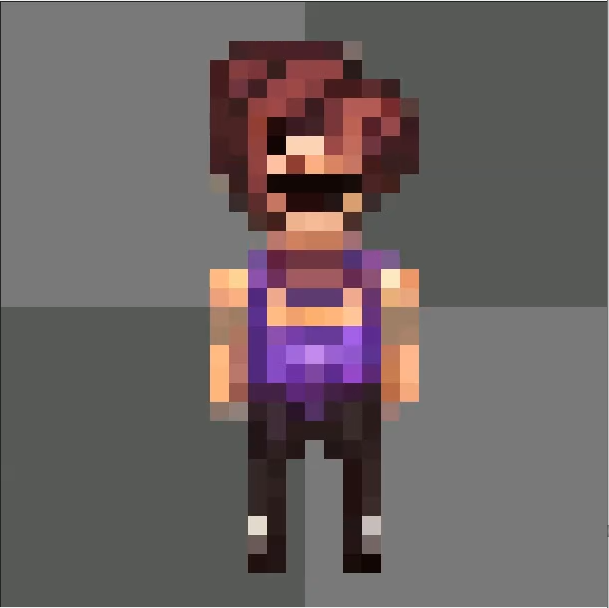
\includegraphics[width=1\linewidth]{figs/pixelLab/dia4/printB.PNG}
        \caption{\small Frame 2 da animação gerada  }
        \label{fig:pixelLabAnimaComparaRodarFrame2}
    \end{subfigure}
    \legend{\small Fonte: Elaborada pela autora, utilizando a ferramenta Pixel Lab.}
\end{figure}

A análise revela que a ferramenta é capaz de gerar animações consistentes se a animação de referência é parecida com o sprite, porém o resultado formado ainda exige ajustes finos, possuindo falhas de pixels e tons de cores não idênticos aos desejados, o que faz com que sua performance na geração não alcance a mesma qualidade comparada às ferramentas descritas nas próximas seções. Apesar disso, assim como a funcionalidade de rotação, a criação de animação baseada em outra animação apresenta grande potencial de otimização do processo em cenário com uma animação base de alta qualidade ou com diversos personagens de tamanho e forma parecidos.


%   ------------------------------------------------------------------------
\FloatBarrier
\subsection{Uso no pós-processamento}
\label{s.pixelLab.edicao}


Um dos principais usos do PixelLab.AI neste projeto foi como ferramenta de pós-processamento, aplicando ajustes finos manuais nos resultados gerados por outras ferramentas de forma que o resultado final já podia ser diretamente aplicado no jogo. A forma de exportação, o editor embutido e o ambiente em pixel art foram funcionalidades que trouxeram eficiência para essa etapa de correções, que é justamente o que falta na maioria das outras ferramentas.

Nessa seção, abordaremos as edições feitas que geraram o resultado final.

Como comentado em seções anteriores, o sprite do personagem Pablo em side view gerado pela ferramenta Gemini Pro (Figura \ref{fig:pixelLabPabloGeminiProSide}) passou por uma correção, onde os tons de cores e o tamanho foram ajustados, comparando o sprite lado a lado com a imagem do mesmo personagem de frente como pode ser visto nas Figuras \ref{fig:pixelLabFixSideViewComparaAntes} e \ref{fig:pixelLabFixSideViewComparaDepois}. Esse processo é extremamente importante, pois durante o jogo, o sprite de um personagem deve ser realmente consistente com os outros sprites daquele personagem, uma vez que haverá transições entre cada uma dessas figuras. Se a consistência não se mantém, em vez de apenas demonstrar um movimento ou mudança de posição, é causado um estranhamento no jogador. Posteriormente, uma nova edição foi realizada para ajustar detalhes como a falta de cabelo na nuca e o formato da orelha. Esse processo é demonstrado na Figura \ref{fig:pixelLabFinalSideView}.

\begin{figure}[htbp]
    \centering
    \caption{\small Comparação do sprite original e sprite gerado pelo Gemini Pro antes da edição}
    \label{fig:pixelLabFixSideViewComparaAntes}
    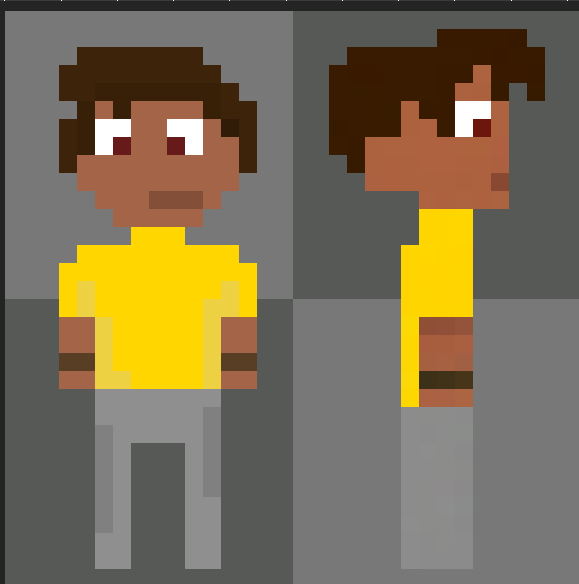
\includegraphics[width=0.4\linewidth]{figs/pixelLab/dia3/comparacao.PNG}
    \legend{\small Fonte: Elaborada pela autora.}
\end{figure}
    
\begin{figure}[htbp]
    \centering
    \caption{\small Comparação do sprite original e sprite gerado pelo Gemini Pro depois da edição}
    \label{fig:pixelLabFixSideViewComparaDepois}
    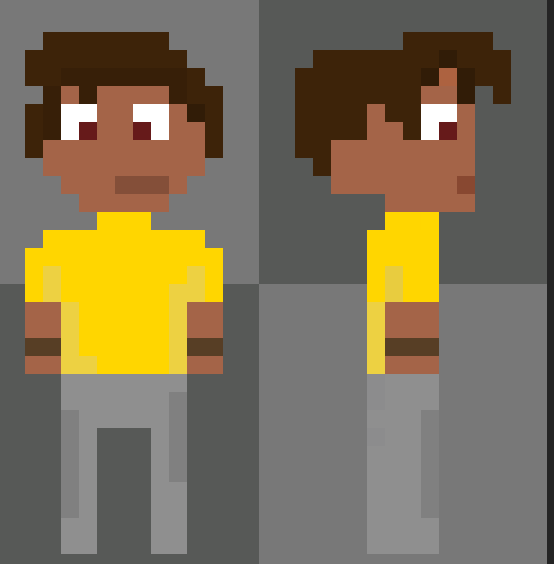
\includegraphics[width=0.4\linewidth]{figs/pixelLab/dia3/fix.PNG}
    \legend{\small Fonte: Elaborada pela autora, utilizando a ferramenta Pixel Lab.}
\end{figure}

\begin{figure}[htbp]
    \centering
    \caption{\small Processo de edição no Pixel Lab do sprite em side view gerado pelo Gemini Pro}
    \label{fig:pixelLabFinalSideView}
    \begin{subfigure}{0.32\linewidth}
        \centering
        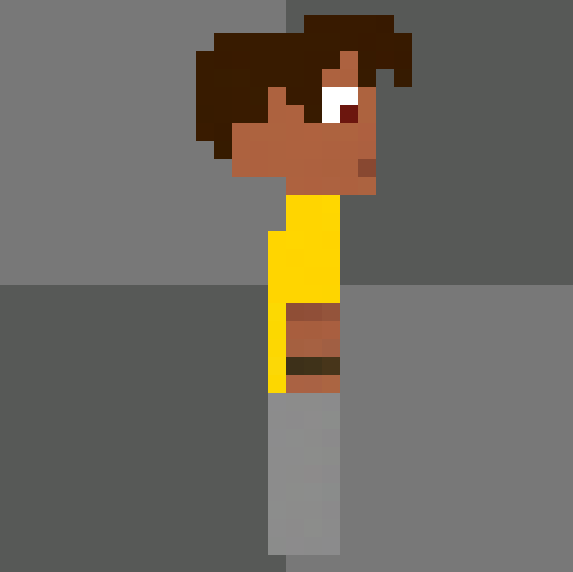
\includegraphics[width=1\linewidth]{figs/pixelLab/dia3/semFix.PNG}
        \caption{\small Antes da edição no Pixel Lab}
        \label{fig:pixelLabFinalSideView1}
    \end{subfigure}
    \begin{subfigure}{0.32\linewidth}
        \centering
        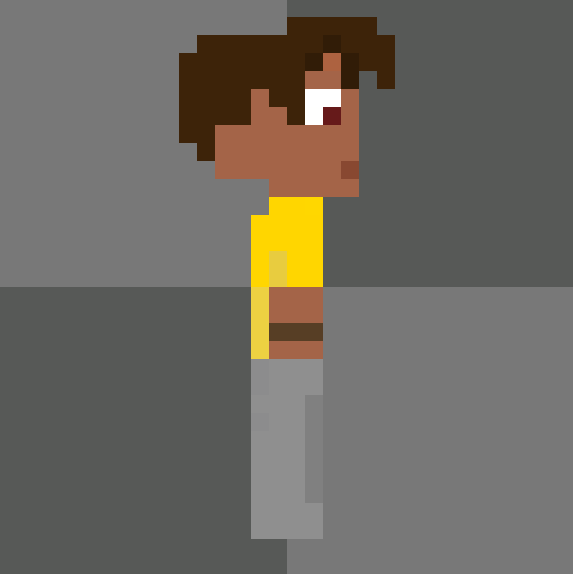
\includegraphics[width=1\linewidth]{figs/pixelLab/dia3/fixGrande.PNG}
        \caption{\small Após a primeira edição no Pixel Lab}
        \label{fig:pixelLabFinalSideView2}
    \end{subfigure}
    \begin{subfigure}{0.32\linewidth}
        \centering
        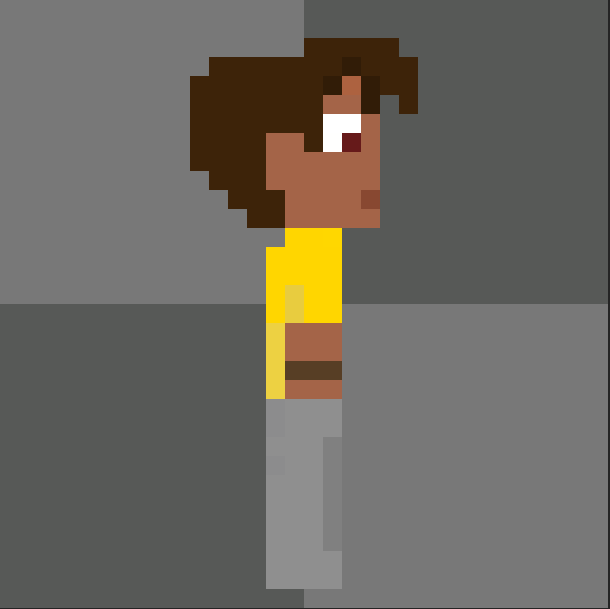
\includegraphics[width=1\linewidth]{figs/pixelLab/dia3/fix_oficial_fundo_igual.PNG}
        \caption{\small Resultado final}
        \label{fig:pixelLabFinalSideView3}
    \end{subfigure}

    \legend{\small Fonte: Elaborada pela autora, utilizando a ferramenta Pixel Lab.}
\end{figure}

Também foram realizados ajustes finos na, anteriormente apresentada, Figura \ref{fig:pixelLabPabloGeminiProCostas}, que mostra o sprite do personagem Pablo de costas gerado pelo Gemini Pro (detalhado na Seção \ref{s.ferramentaB}). O processo foi parecido com o do personagem em side view, usando a visão de frente para corrigir as cores e o tamanho da imagem. Além disso, pixels do que antes era o fundo branco foram apagados, mantendo a imagem com um fundo transparente. Esse processo pode ser verificado na Figura \ref{fig:pixelLabFinalBackView}.

\begin{figure}[htbp]
    \centering
    \caption{\small Processo de edição no Pixel Lab do sprite em back view gerado pelo Gemini Pro}
    \label{fig:pixelLabFinalBackView}
    \begin{subfigure}{0.45\linewidth}
        \centering
        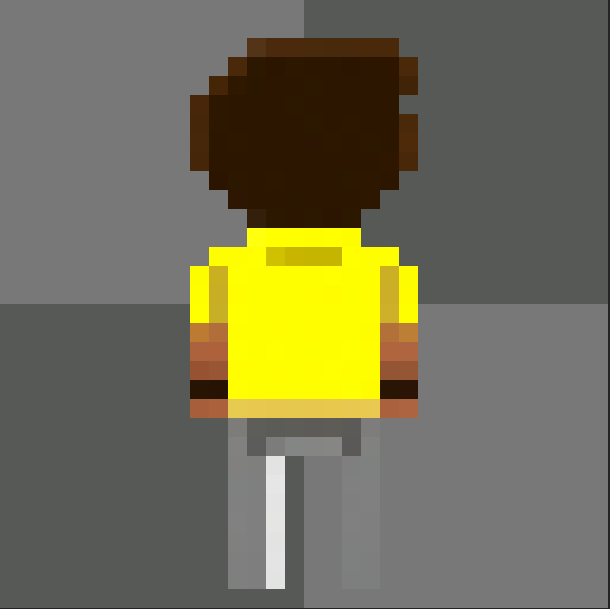
\includegraphics[width=1\linewidth]{figs/pixelLab/dia3/back_sem_fix.PNG}
        \caption{\small Antes da edição no Pixel Lab}
        \label{fig:pixelLabFinalBackView1}
    \end{subfigure}
    \begin{subfigure}{0.45\linewidth}
        \centering
        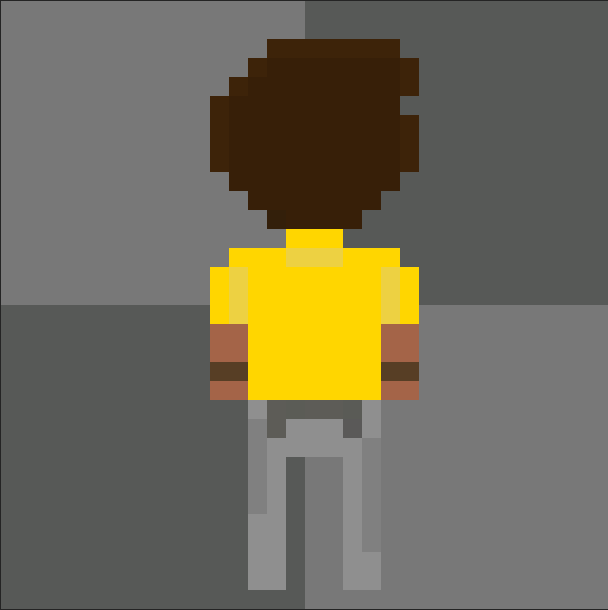
\includegraphics[width=1\linewidth]{figs/pixelLab/dia3/back_fix.PNG}
        \caption{\small Resultado final}
        \label{fig:pixelLabFinalBackView2}
    \end{subfigure}


    \legend{\small Fonte: Elaborada pela autora, utilizando a ferramenta Pixel Lab.}
\end{figure}

Os ajustes finos feitos no sprite sheet da porta abrindo em side view (Figura \ref{fig:pixelLabPortaViduSideView}) gerada pelo Vidu (detalhado na Seção \ref{s.vidu}) foram parcialmente parecidos com os anteriores, usando o sprite da porta fechada (Figura \ref{fig:pixelLabPortaSideView} para corrigir a altura, além de retirar qualquer pixel branco. Além disso, a moldura da porta (presente no sprite) foi fixada na mesma posição em todos os quadros, pois a moldura deve permanecer igual sem se mover mesmo quando a porta é aberta. Após isso, para cada um dos quadros, foi apagada a maçaneta ainda ligada à moldura, pintada novamente aquela parte da porta e desenhada uma nova maçaneta no canto correto. Após 12 quadros (dos 31 totais), foi observada que a porta praticamente não ficava mais aberta, com a maior parte dos outros frames igual ou muito similares. Dessa forma, os frames restantes foram apagados para não ocorrer perda de tempo em mudanças insignificantes.

A parte mais complexa do processo foi fazer novamente a maçaneta, pois era necessário entender o formato correto que ela ficaria dependendo do ângulo e como representar essa forma através dos tons de cores. Apesar disso, foi uma tarefa muito mais simples e rápida do que fazer a porta inteira do zero múltiplas vezes com cada frame tendo apenas pequenas modificações. O resultado desse processo final de edição pode ser verificado na Figura \ref{fig:pixelLabFinalPortaSideView}.

\begin{figure}[htbp]
    \centering
    \caption{\small Processo de edição no Pixel Lab do sprite sheet da porta gerado pelo Vidu}
    \label{fig:pixelLabFinalPortaSideView}
    \begin{subfigure}{0.45\linewidth}
        \centering
        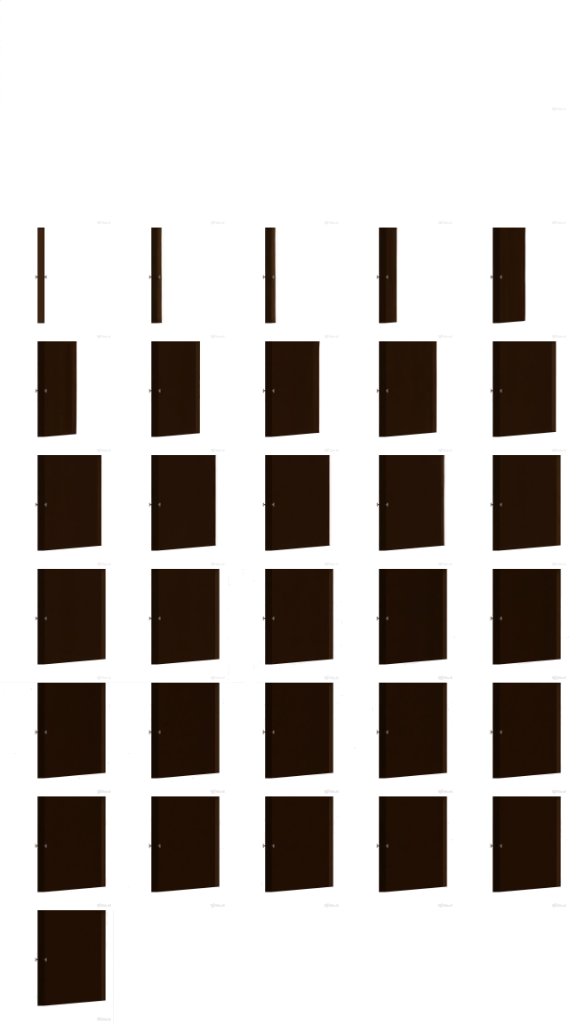
\includegraphics[width=1\linewidth]{figs/vidu/Pixilart/porta_sprite_sheet_pixel.png}
        \caption{\small Antes da edição no Pixel Lab}
        \label{fig:pixelLabFinalPortaSideView1}
    \end{subfigure}
    \begin{subfigure}{0.45\linewidth}
        \centering
        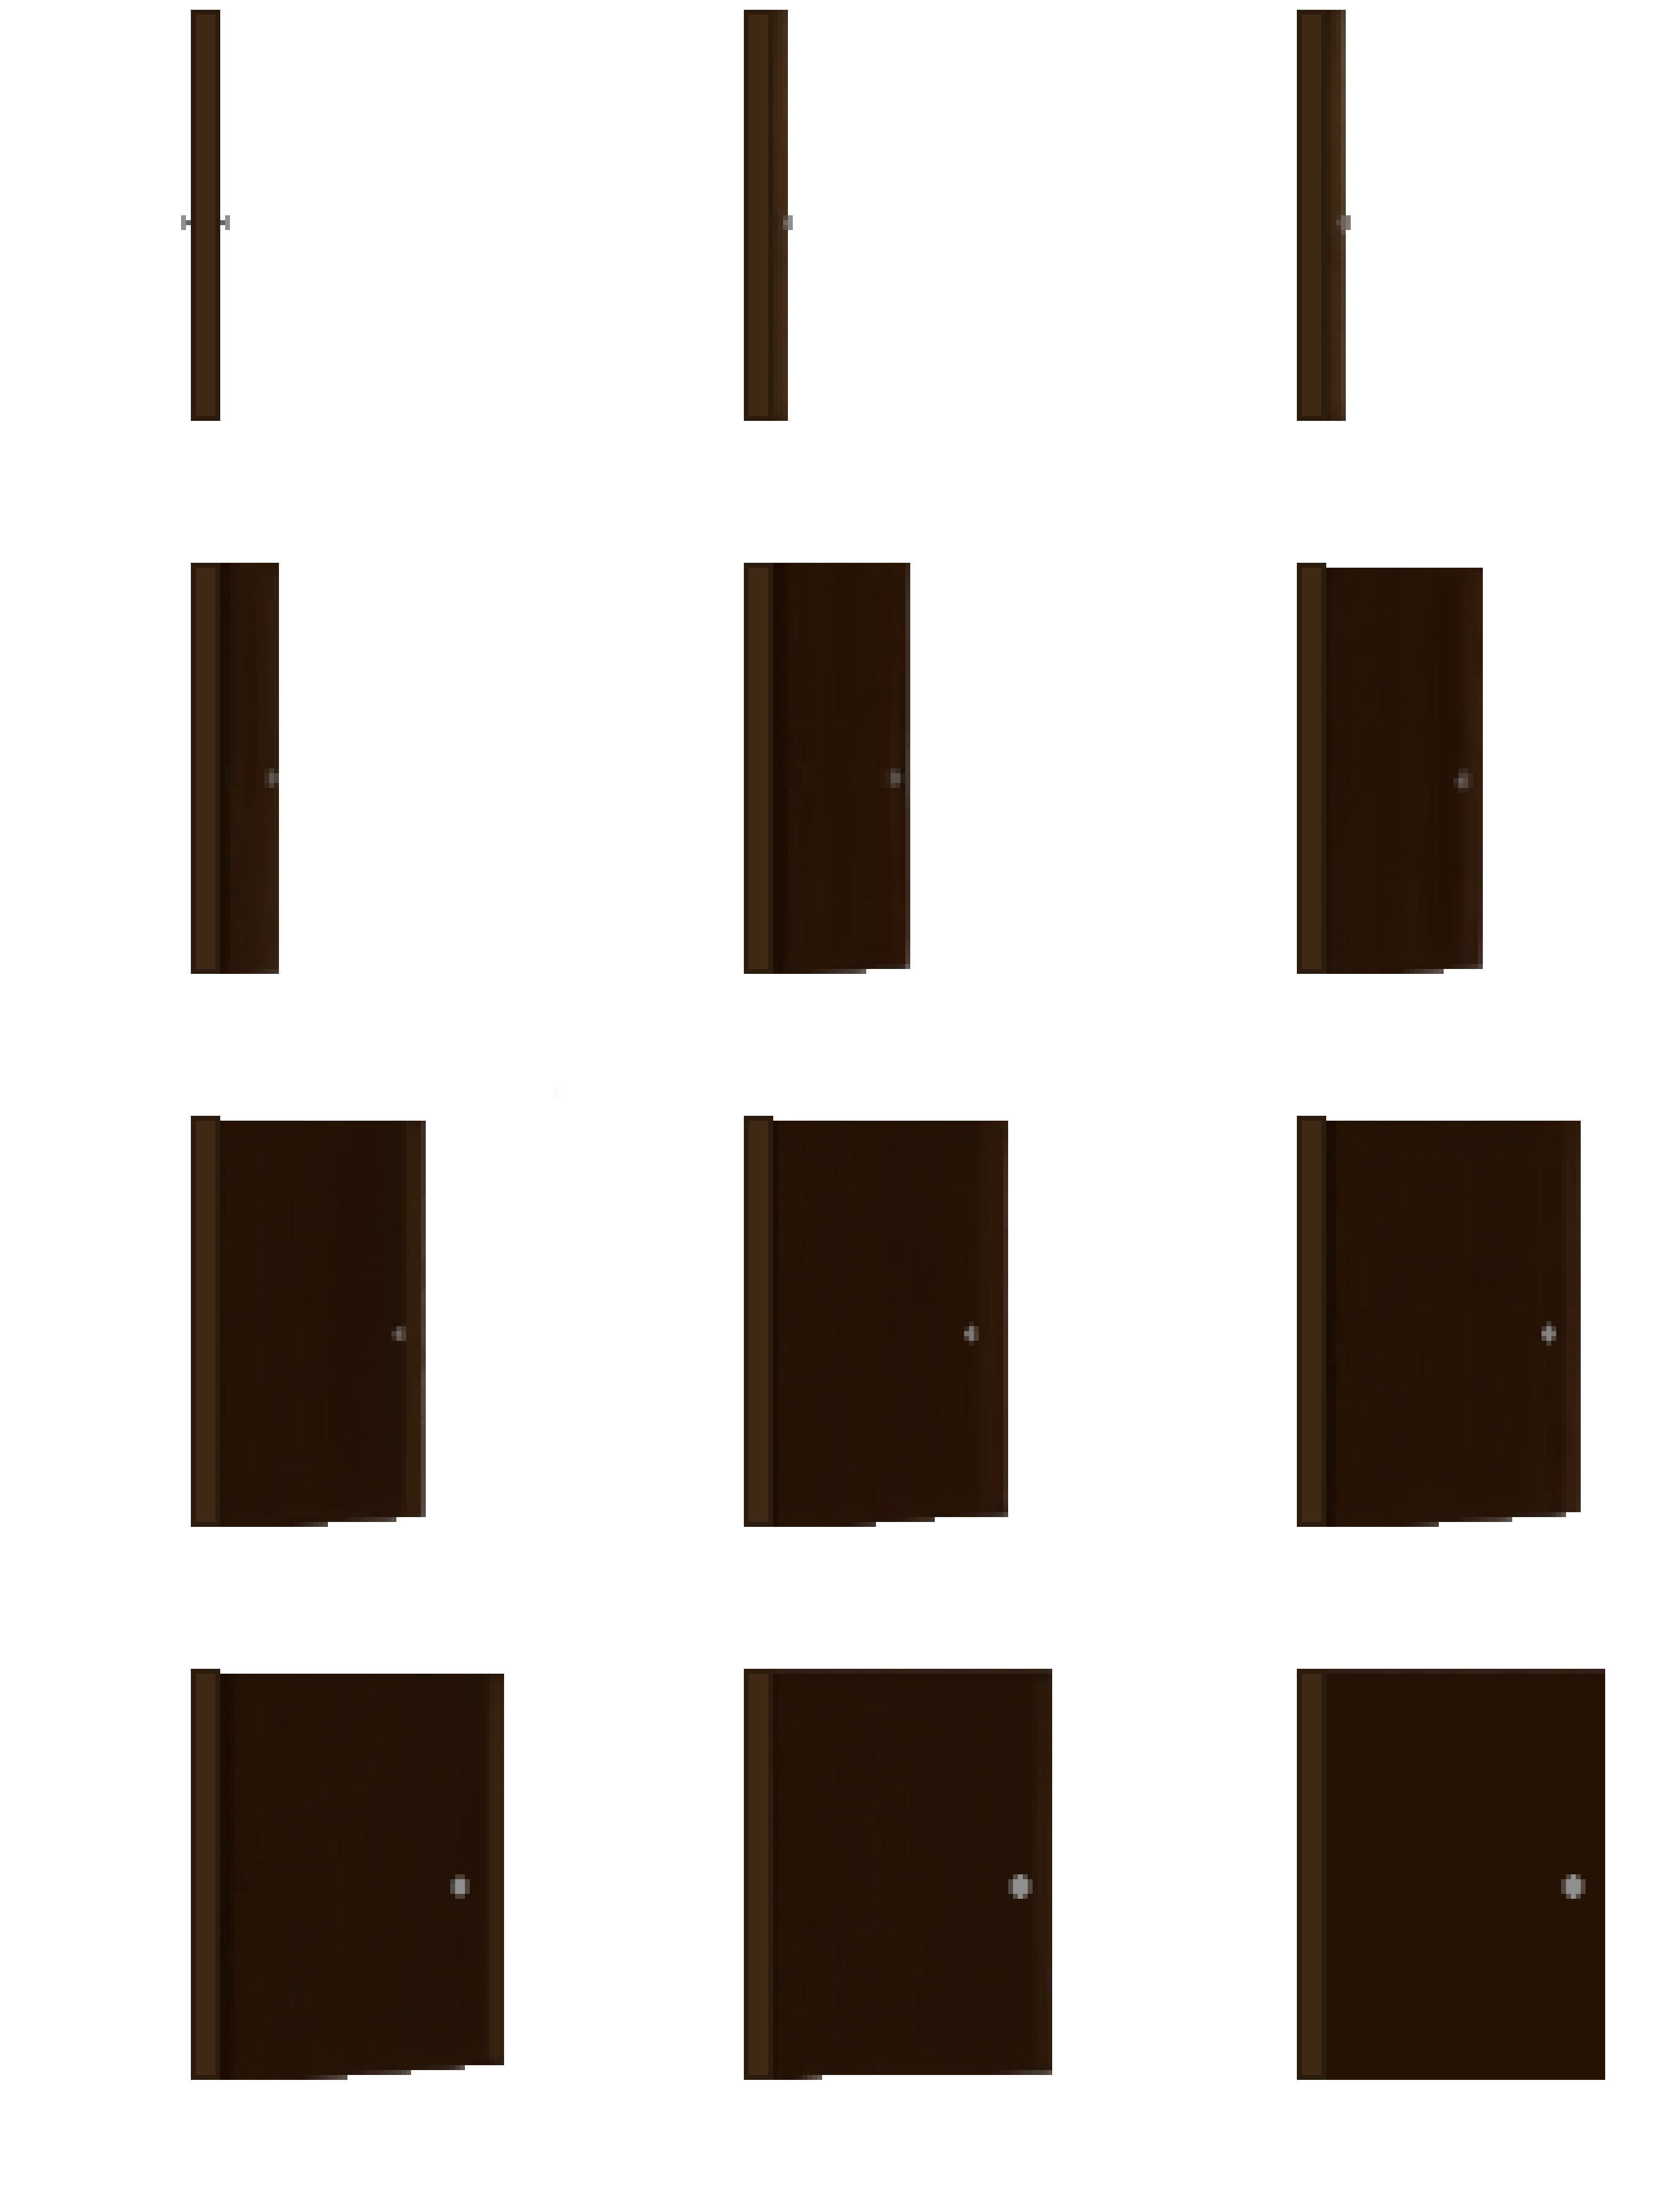
\includegraphics[width=1\linewidth]{figs/pixelLab/final/side_door_pixel_vidu.png}
        \caption{\small Resultado final}
        \label{fig:pixelLabFinalPortaSideView2}
    \end{subfigure}


    \legend{\small Fonte: Elaborada pela autora, utilizando a ferramenta Pixel Lab.}
\end{figure}